\providecommand{\main}{../../../..}
\documentclass[\main/dresen_thesis.tex]{subfiles}

\begin{document}
  \paragraphNewLine{Scanning Electron Microscopy}
    The double layers with varied spacer thickness are characterized qualitatively by scanning electron microscopy.
    A Neon Zeiss 40 (\refsec{ch:instruments:laboratoryInstruments:sem}) is operated to obtain top-view and cross-sectional micrographs of each sample.
    For the cross-sectional views, the samples are cut on two opposing sides with a diamond cutter and broken downward.
    The micrographs are measured at $5 \unit{kV}$ and the data from the back-scattering electron detector is shown.

  \paragraphNewLine{X-Ray Reflectometry}
    Using a Bruker D8 Advanced at the \textsc{Forschungszentrum J\"ulich} (\refsec{ch:instruments:laboratoryInstruments:xrr}), XRR of all double layers is measured.
    The samples are measured with a Cu-K$\alpha$ source ($\lambda \eq 1.54 \unit{\angstrom}$) and a $q$-range of $0 - 0.35 \unit{\angstrom^{-1}}$ is evaluated by measuring $2 \theta \eq 0^\circ - 5 ^\circ$ in $0.01 ^\circ$ steps over an integrated time of approximately $1 \unit{h}$.
    To perform the footprint correction (\refsec{ch:methods:xrr}) of the sample, the collimation slit of the instrument with $0.2 \unit{mm}$ and samples width of $10 \unit{mm}$ is considered.
    An equidistributed beam intensity profile is assumed for the correction.

  \paragraphNewLine{Polarized Neutron Reflectometry}
    The samples DL-0.125\%, DL-0.25\%, DL-1.25\% and DL-2.5\% are measured by polarized neutron reflectometry on the D17 (\refsec{ch:lss:d17}) at the Institute Laue-Langevin.
    The instrument is operated in the time-of-flight mode and the samples are measured at three incident angles of $0.50^\circ ,\, 1.80^\circ ,\, 4.00^\circ$ each to discuss a $q$-range of $0 - 0.2 \unit{\angstrom^{-1}}$.
    The data is reduced with the COSMOS software, which is maintained by the instrumental scientists \cite{Gutfreund_2018_Towar}.
    Each sample is measured after zero-field cooling at $\mathrm{T} \eq 5 \unit{K}$ with polarized neutrons at a guide field of $B \eq 10 \unit{mT}$, then at saturation of $6 \unit{T}$ and finally at a negative field of $-100 \unit{mT}$.

    \begin{figure}[tb]
      \centering
      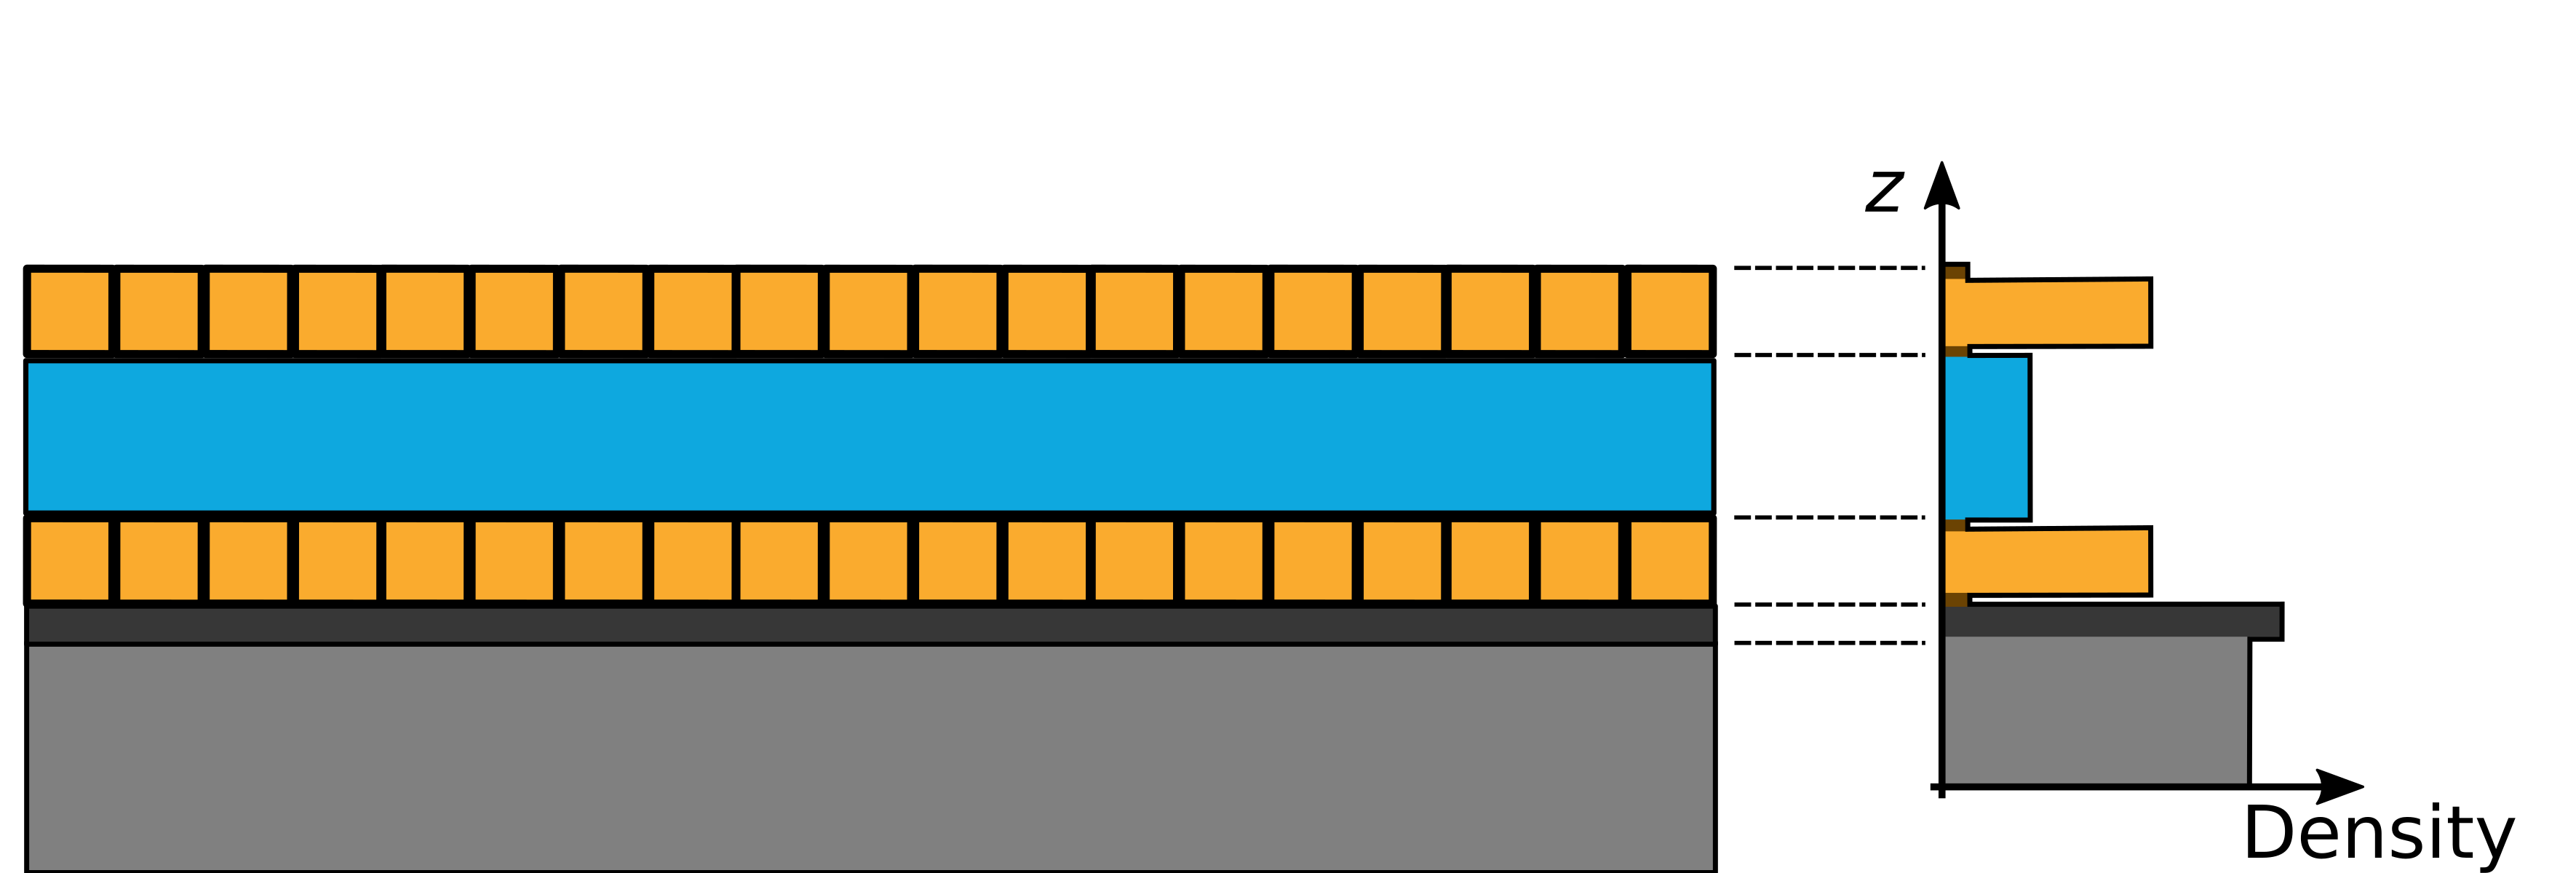
\includegraphics{doublelayers_structure_verticalModel}
      \caption{\label{fig:doubleLayers:characterization:doublelayerModel}Depiction of the double layer model used to simulate the expected half-polarized reflectivities for specific magnetic configurations in PNR.}
    \end{figure}
    Expected half-polarized reflectivities are simulated using the scattering length density profile model depicted in \reffig{fig:doubleLayers:characterization:doublelayerModel}.
    The SLD, thickness and roughness of the substrate, silicon dioxide layer, two nanoparticle layers, as well as the oleic acid surfactant layers is used as determined for the monolayer prepared from the same nanocubes in \refsec{sec:monolayers:structure:verticalModel}.
    The PMMA layer in-between is simulated with a scattering length density of $1.059 \cdot \unit{10^{-6} \angstrom^{-2}}$, with varied thickness.
    For the simulation, the roughness between PMMA and oleic acid is neglected.
    An instrumental resolution is included in the simulation with $\sigma_\theta \eq 0.3 \unit{mrad}$ and $\sigma_\lambda / \lambda \eq 2.5 \%$.
    
  \paragraphNewLine{Vibrating Sample Magnetometry}
    The macroscopic magnetization of the double layers with varied spacer thickness are each measured field- and temperature-dependent using a PPMS Evercool II (\refsec{ch:instruments:laboratoryInstruments:vsm}).
    Each sample is cut with a diamond cutter to a size of approximately $5 \times 5 \unit{mm^2}$ and stuck on a quartz sample holder by a low temperature varnish (GE 7031).

    The samples are measured field-dependent in a range of $\pm 9 \unit{T}$ at $300 \unit{K}$ and $10 \unit{K}$ with a sweeping rate of $5 \unit{mT \, s^{-1}}$.
    The measurements at $10 \unit{K}$ are performed after cooling in a field of $10 \unit{mT}$.
    The sample magnetization is furthermore measured temperature-dependent after zero-field cooling and field cooling at $10 \unit{mT}$ from $10 \unit{K}$ to $350 \unit{K}$ while warming the sample with a rate of $1.5 \unit{K \, s^{-1}}$.

    As the samples vary slightly in size, the mass of the silicon wafers is measured by a precision scale to estimate the measured area. As the thickness of the silicon does not vary, but is by a micrometer scale measurably given by $0.52 \unit{mm}$, and as the nanoparticle and PMMA layer only contributes a mass in the order of $\musf g$, the sample mass is directly proportional to the surface area.
    The determined masses of the samples are tabulated in \reftab{tab:doubleLayers:layerCharacterization:ppmsMasses}.
    Using the silicon mass density $\rho_\mathrm{Si} \eq 2.32 \unit{g \, cm^{-3}}$, the measured magnetization is scaled to the sample area by
    \begin{align}
      \bar{M} \eq \frac{\rho_\mathrm{Si} d_\mathrm{Si}}{m_\mathrm{sample}} M.
    \end{align}
    The sample susceptibility and spontaneous magnetization are obtained from the room temperature magnetization by a linear fit in the range of $5 - 9 \unit{T}$ and compared between the double layer samples.

    \begin{table}[!htbp]
      \centering
      \caption{\label{tab:doubleLayers:layerCharacterization:ppmsMasses}Mass of the samples used for the VSM measurements.}
      \begin{tabular}{ l | l}
        \rule{0pt}{2ex} \textbf{Sample}  & $m \, / \unit{mg}$ \\
        \hline
        \rule{0pt}{2ex} DL-0.125\%   & $29.55(2)$ \\
        \rule{0pt}{2ex} DL-0.25\%    & $27.44(2)$ \\
        \rule{0pt}{2ex} DL-1.25\%    & $26.73(2)$ \\
        \rule{0pt}{2ex} DL-2.5\%     & $29.51(2)$ \\
        \rule{0pt}{2ex} DL-5\%       & $30.27(2)$ \\
        \hline
      \end{tabular}
    \end{table}

\end{document}